\documentclass[14pt]{extarticle}
\usepackage[utf8]{inputenc}
\usepackage[T2A,T1]{fontenc} 
\usepackage[russian]{babel}
\usepackage{graphicx}
\usepackage{geometry}
\usepackage{titlesec}
\usepackage{amsmath}
\usepackage{subcaption}
\usepackage{enumitem}
\usepackage{multicol}

\graphicspath{ {images/} }

\geometry{
a4paper,
left=40pt,
top=40pt,
right=40pt,
bottom=40pt
}

\begin{document}
\linespread{0.9}
%\titleformat{<command>}[<shape>]{<format>}{<label>}{<sep>}{<before-code>}[<after-code>]
\titleformat{\paragraph}{\centering}{}{0em}{}
\setlength{\columnsep}{20pt}
\twocolumn

\begin{figure}[h]
    \begin{subfigure}[h]{0.8\linewidth}
        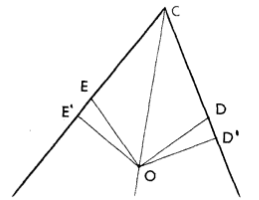
\includegraphics[width=\textwidth]{1.1}
        \caption{}
    \end{subfigure}
    \begin{subfigure}[h]{0.8\linewidth}
        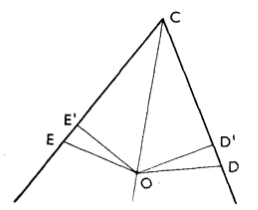
\includegraphics[width=\textwidth]{1.2}
        \caption{}
    \end{subfigure}
        \caption{}
\end{figure}


Мы хотим предоставить читателям в качестве упражнения найти ошибку в приведенном выше рассуждении.

Следует заметить, что число экзаименующихся, правильно решивших эту задачу (и аналогичные задачи других вариантов) было сравнительно невелико: ее решил, примерно, 1 человек из 9.
\paragraph{Задача 3}

Решение первого уравнения данной системы:
\[\cos x - \cos 13x = 0\]
или
\[2\sin 7x \sin 6x = 0\]
дает две серии значений
\begin{enumerate}[label=\alph*)]
    \item \(x=\frac{1}{7}n\pi \quad (n=0, \pm1, \pm2,\dots)\) \label{range:a}
    \item \(x=\frac{1}{6}m\pi \quad (m=0, \pm1, \pm2,\dots)\) \label{range:b}
\end{enumerate}

Отбирая из этих значений те, которые удовлетворяют неравенству \(|x| < 3\), находим:
\begin{enumerate}[label=\alph*)]
    \item \(x = \frac{1}{7} n \pi, \quad |n| \leq 6,\)
    \item \(x = \frac{1}{6} m \pi, \quad |m| \leq 5.\)
\end{enumerate}

Теперь мы должны выбрать те значения х, которые удовлетворяют второму уравнению системы. Это уравнение можно представить в виде:
\begin{align*}
1 =\sin 5x + \cos 2x =\\
=\sin 5x + \sin\left(\frac{\pi}{2} + 2x\right) =\\
=2\sin\left(\frac{7x}{2} + \frac{\pi}{4}\right)\cos\left(\frac{3x}{2} - \frac{\pi}{4}\right)
\end{align*}                

Подставим в него сначала серию \ref{range:a}. Поскольку \(7x =n\pi \quad(|n| \leq 6)\), то должно выполняться равенство:
\begin{equation}\label{eq:1}
\sin\left(\frac{n\pi}{2}+\frac{\pi}{4}\right)\cos\left(\frac{3n\pi}{14}-\frac{\pi}{4}\right)=\frac{1}{2}
\end{equation}
 
Так как \(\sin\left(\frac{n\pi}{2}+\frac{\pi}{4}\right) = \pm\frac{\sqrt{2}}{2}\), то    \(\cos\left(\frac{3n\pi}{14}-\frac{\pi}{4}\right)=\pm\frac{\sqrt{2}}{2}\) и, следовательно, \(\frac{3n\pi}{14}-\frac{\pi}{4}\) должно отличаться от \(\frac{\pi}{4}\) на число кратное \(\frac{\pi}{2}\). Однако \(\frac{3n\pi}{14}=\frac{3n}{7}\frac{\pi}{2}\), так что \(\frac{3n}{7}\) должно быть целым. При ограничении \(|n| \leq 6\) это имеет место лишь при \(n=0\). Подставляя значение \(n=0\) в уравнение (\ref{eq:1}), убеждаемся, что оно ему удовлетворяет. Итак, из серии \ref{range:a} решением является только \(x=0\).

Проверим теперь серию \ref{range:b}{}. Представив второе уравнение данной системы в виде
\begin{equation}\label{eq:2}
\sin5x = 1 - \cos2x = 2\sin^2 x,
\end{equation}
замечаем, что \(\sin 5x\) должен быть неотрицательным, то есть угол \(5x=\frac{5}{6}m\pi \quad (|m|\leq 5)\) заключен в первых двух четвертях. Подставляя в выражение \(\frac{5}{6}m\pi\) возможные целые значения m от -5 до +5, устанавливаем, что проверке подлежат только шесть из них: \(m=0, 1, 3, 5; -2, -4\). Вычисляя при этих значениях левую и правую части уравнения \ref{eq:2}, получаем таблицу:

\begin{tabular}{ |c|c|c|c|c|c|c| } 
    \hline
    m & 0 & 1 & 3 & 5 & -2 & -4 \\
    \(\sin{\frac{5m\pi}{6}}\) & 0 & \(\frac{1}{2}\) & 1 & \(\frac{1}{2}\) & \(\frac{\sqrt{3}}{2}\) & \(\frac{\sqrt{3}}{2}\) \\
    \hline
\end{tabular}

% sin
% m
% 5тл
% 6
% 2 sin*
% тл
% 6
% из которой получаем искомые решения:
% m=0, 1, 5, т. е.
% 5л
% x= 0, 6
% (3)
% Три значения (3) и дают полное ре-
% шение задачи, так как решение серии
% (а) давало значение х=0, уже вклю-
% ченное в (3).
% Отметим, что таким же образом, пу-
% тем перебора, можно проверить и се-
% рию (а).
% При решении этой задачи характер-
% ной ошибкой было следующее: мно-
% гие забывали, что решение должно
% удовлетворять всем условиям зада-
% чи одновременно, а зачастую
% просто не понимали этого. Некоторые
% ограничивались тем, что решали одно
% из уравнений и совершали отбор ре-
% шений по неравенству, другие ком-
% бинировали уравнения и решали в
% конце концов также лишь одно урав-
% нение, не эквивалентное предложен-
% ной системе.
% З адача 4
% Пусть ABCD -- данный четырех-
% угольник, AВ=V5. Прямоугольные
% проекции любого многоугольника на
% параллельные плоскости равны меж-
% ду собой; поэтому проведем плоскости
% P4 и Р2 параллельные исходным пло-
% скостям, через вершину А и
% в дальнейшем будем говорить о про-
% екциях четырехугольника именно на
% эти плоскости.
% Для каждой точки М пространства
% мы будем обозначать через М1,М2 и
\end{document}